\section{Energieübertragung}\label{sec:energie}
In diesem Kapitel wird aufgezeigt, wie die Energie übertragen werden soll. Zudem werden die Schaltung auf der Primär- und der Sekundärseite entworfen.

\subsection{Konzept}
In der Abbildung \ref{fig:konzept_energie} sind die wichtigsten Komponenten der induktiven Energieübertragung aufgeführt. Rot umrandet sind die Komponenten, die entwickelt werden müssen. Die Spannungsquelle und der Treiber für den Motor sind extern. Der Treiber bestimmt die zu übertragende Leistung von 300W und einer Gleichspannung von 48V.

\begin{figure}[h]
	\centering
	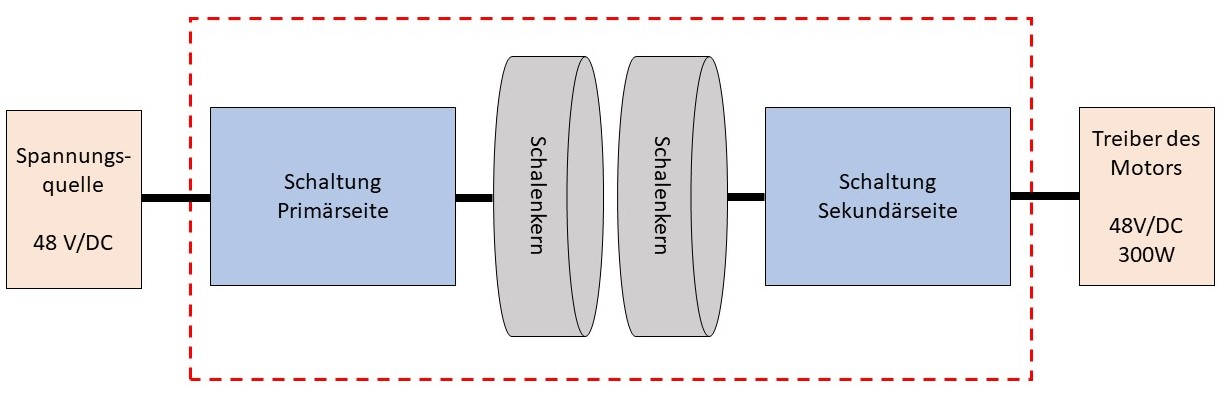
\includegraphics[width=1\linewidth]{konzept_energie}
	\caption{Konzept der induktiven Energieübertragung}\label{fig:konzept_energie}
\end{figure}

Die beiden Schalenkerne werden benötigt, um einen guten Kopplungsfaktor zu erreichen. Es sind Ferritkerne, welche aus dem Material BFM8 bestehen und eine Anfangspermeabilität $ \mu_{i} $ von 2400 aufweisen.\\ Die Schaltung auf der Primärseite hat die Aufgabe aus der Gleichspannung eine gepulste Spannung zu erzeugen, da keine konstante Spannung an der Spule anliegen darf. Wäre dies nicht der Fall, könnte man keine Energie übertragen. Denn das Magnetfeld der Spule würde sich nicht ändern und es würde kein Strom in die zweite Spule induziert. \\
Auf der sekundären Seite wird wieder eine gepulste Spannung generiert. Aus dieser gepulsten Spannung soll die Sekundärschaltung wieder eine Gleichspannung kreieren.

\paragraph{Auswahl der Schaltungstopologie}
Für die Energieübertragung kommen verschiedene Typologien zu Frage. Der Flyback bringt interessante Vorteile mit sich. Im Vergleich zu anderen Schaltungen, welche eine galvanische Trennung beinhalten, benötigt er weniger Bauteile. Zusätzlich eignet sich die Schaltung für einen Leistungsbereich bis zu ca. 500W. Im Gegensatz zum Resonanzwandler muss der benötigte Transformator bestimmte Anforderungen erfüllen, da er gleichzeitig als Energiespeicher eingesetzt wird. Da es für einen Prototypen von Vorteil ist, möglichst wenig Bauteile zu verwenden, fiel der Entscheid auf den Flyback-Converter. \cite{bachelor} \cite{speerwandler}

In der Abbildung \ref{fig:konzept_flyback} wird die Schaltung des Flyback-Converters aufgesplittet in die Primärschaltung, die Sekundärschaltung und die Schalenkerne. Die Primärseite besteht hauptsächlich aus dem MOSFET und dem Snubber-Glied. Die beiden Schalenkerne bilden den Speichertransformator, der für den Flyback benötigt wird. Die Sekundärschaltung ist ein Gleichrichter, welcher aus einer Schottky-Diode und einem Kondensator gebildet wird.
\begin{figure}[h]
	\centering
	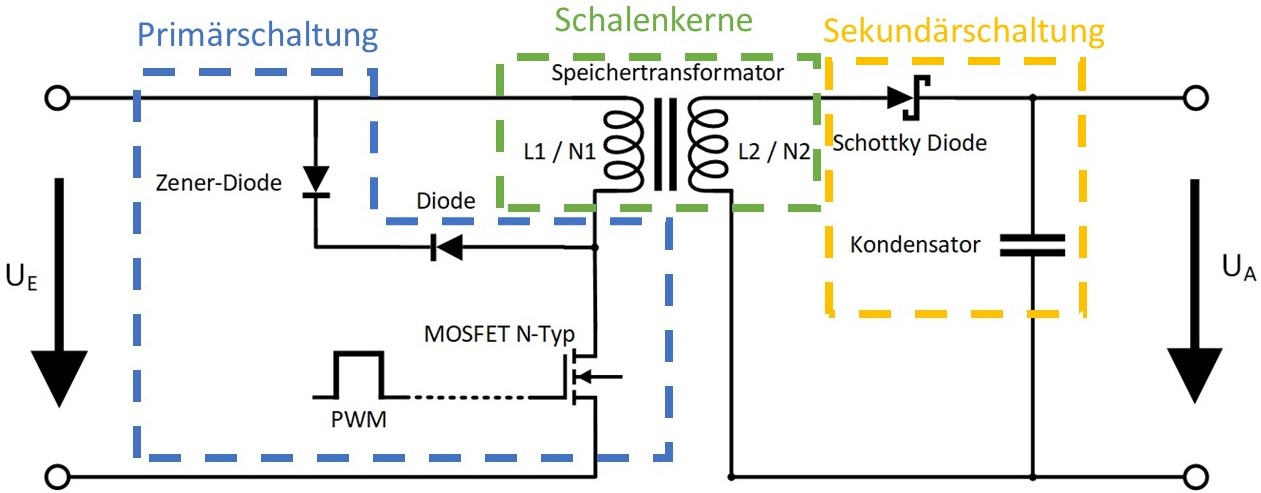
\includegraphics[width=0.9\linewidth]{konzept_flyback}
	\caption{Unterteilung der Flyback Schaltung}\label{fig:konzept_flyback}
\end{figure}


\subsection{Dimensionierung Flyback-Converter}

Um den Flyback-converter simulieren und später in einem Testaufbau realisieren zu können, müssen die wichtigsten Komponenten ausgelegt werden. In diesen Abschnitt wird die Dimensionierung der Induktivität des Speichertransformators, des MOSFET, der Schottky-Diode und der Snubber-Schaltung erklärt. Die genauere Dimensionierung des Speichertransformators wird im Abschnitt  \textbf{\ref{sec:simulation} \nameref{sec:simulation}} genauer beschrieben.

\paragraph{Berechnung der Induktivität}
Ein wichtiger Wert, um den Speichertransformator zu dimensionieren, ist die Induktivität. Mit den beiden Formeln \ref{eq:energie} und \ref{eq:Leistung} kann die übertragene Leistung $ P $ beschreiben werden. \cite{lea}

\begin{equation}\label{eq:zusammen}
P = \frac{1}{2} \cdot L \cdot \left (\frac{U_{E}}{L}\cdot a \cdot T_{p}\right ) ^{2} \cdot f_{p}
\end{equation}

Die Gleichung \ref{eq:zusammen} lässt sich nun nach der gesuchten Induktivität $ L $ umformen.

\begin{equation}\label{eq:induktivität}
L = \frac{a^{2}\cdot U_{E}\!^{2}\cdot T_{p}}{2 \cdot P}
\end{equation}

Mit einem Tastverhältnis $ a $ von 0.5, einer Eingangspannung $ U_{E} $ von 48V und der übertragenen Leistung $ P $ von 300W wird die Induktivität berechnet. Die Periodendauer $ T_{p} $ ist variabel.

\begin{equation}\label{eq:induktivität_berechnet}
L = \frac{0.5^{2}\cdot 48\mathrm{V}^{2}\cdot T_{p}}{2 \cdot 300\mathrm{W}}
\end{equation}

In der Tabelle \ref{tab:induktivität} sind die berechneten Resultate der Induktivität in Abhängigkeit zur Schaltfrequenz aufgeführt. Die Berechnungen geben Aufschluss darüber, dass die Induktivität kleiner werden muss, wenn die Frequenz erhöht wird. Dies wird auch mit der Formel \ref{eq:strom} deutlich. In der Formel ist das Tastverhältnis, der Strom und die Spannung konstant. Wenn nun die Frequenz steigt, wird die Periodendauer kleiner und die Induktivität muss dementsprechend gesenkt werden.

\begin{table}[H]
	\centering
	\begin{tabular}{>{\tt}C{2.3cm}|  L{3cm}} 
		\normalfont\textbf{Frequenz} & \normalfont\textbf{Induktivität} \\ \hline\hline 
		10 kHZ & \SI{9.6e-05}{H}      \\ \hline
		20 kHZ & \SI{4.8e-05}{H}      \\ \hline
		30 kHZ & \SI{3.2e-05}{H}      \\ \hline
		40 kHZ & \SI{2.4e-05}{H}      \\ \hline
		50 kHZ & \SI{1.9e-05}{H}      \\ \hline
	\end{tabular}
\caption{Induktivität in Abhängigkeit der Schaltfrequenz }
\label{tab:induktivität}
\end{table}

\paragraph{Auslegung des MOSFET}
Die maximale Drain-Source-Spannung $ U_{DS} $ und der maximale Drain-Strom $ I_{D} $ sind wichtige Kenngrössen für die Auswahl des MOSFETs. Die grösste Spannung $ U_{DSmax} $, mit welcher der MOSFET belastet wird, berechnet sich mit der Formel \ref{eq:sperrspannung_mosfet}. Die Drain-Source-Spannung muss auf jeden Fall grösser $ U_{DSmax} $ gewählt werden.\cite{speerwandler}
\begin{equation}\label{eq:sperrspannung_mosfet}
U_{DSmax} = U_{e} + U_{a} \cdot \frac{N1}{N2}
\end{equation}
\begin{equation}\label{eq:sperrspannung_mosfet_berechnet}
U_{DSmax}= 48\mathrm{V} + 48\mathrm{V} \cdot 1 = 96\mathrm{V}
\end{equation}

\paragraph{Auslegung der Ausgangsdiode}
Die Sperrspannung $ U_{R} $ der Schottky-Diode muss folgendermassen ausgelegt werden.\cite{speerwandler}
\begin{equation}\label{eq:sperrspannung_diode}
U_{R} = U_{a} + U_{e} \cdot \frac{N2}{N1} = 48\mathrm{V} + 48\mathrm{V} \cdot 1 = 96\mathrm{V}
\end{equation}

\paragraph{Auslegung  Snubber-Schaltung}
Im Kapitel \textbf{\ref{sec:Grundlagen} \nameref{sec:Grundlagen}} wurden zwei Snubber Schaltungen vorgestellt. Da der Aufbau mit einer Zener-Diode und einer Diode (Abbildung \ref{fig:Flyback_zehner}) effizienter und zusätzlich unabhängig von der Streuinduktivität ist, ist diese Topologie gewählt worden. Die Durchbruch-Spannung $ U_{Z} $ der Zener-Diode kann mit folgenden zwei Bedingungen festgelegt werden. \cite{bachelor}  

\begin{equation}\label{eq:sperrspannung_zener1}
U_{Z} < U_{DS} - U_{E}
\end{equation}
\begin{equation}\label{eq:sperrspannung_zener1_berechnet}
U_{Z} <  150\mathrm{V} - 48\mathrm{V}  = 102\mathrm{V}
\end{equation}
\begin{equation}\label{eq:sperrspannung_zehner2}
U_{Z} > (U_{A} + U_{F}) \cdot \frac{N_{1}}{N_{2}}
\end{equation}
\begin{equation}\label{eq:sperrspannung_zehner2_berechnet}
U_{Z} >(48\mathrm{V} + 0.7\mathrm{V}) \cdot 1 = 48.7\mathrm{V}
\end{equation}
Die Durchbruch-Spannung darf also maximal 102 V betragen und mindestens 48.7 V.

\subsection{Simulation}\label{sec:simulation}
Um die dimensionierten Werte zu überprüfen und dementsprechend anzupassen, sind zwei Simulationen erstellt worden. Mit dem Simulationstool FEMM kann der Speichertrafo genauer betrachtet werden. Die Schaltung des Flyback-Converters ist im LTspice aufgebaut.

\paragraph{FEMM}
FEMM ist ein Simulationstool mit dem elektromagnetische Probleme im zweidimensionalen Bereich gelöst werden können. Der Speichertransformator ist im FEMM achsensymmetrisch aufgebaut. Er besteht aus den zwei Ferrit-Schalenkerne. Diese sind anhand des Datenblattes aufgezeichnet. Die Anfangspermeabilität $ \mu_{i} $ des Ferrits beträgt 2400 $ \frac{H}{m} $ und die Sättigungsflussdichte ist 490 mT. In der ersten Simulation wird ermittelt, wie viele Windungen für den Speichertransformator benötigt werden. Mit der darauffolgenden Simulation wird der Kopplungsfaktor berechnet. 

Damit der Transformator mit der benötigten Induktivität aufgebaut werden kann, muss die Anzahl Windungen bekannt sein. Die Resultate der Simulation für verschiedene Frequenzen und Distanzen sind in der Tabelle \ref{tab:windungen} aufgeführt. Um die simulierten Werte zu vergleichen sind in der zweiten Spalte die berechneten Resultate aus der Tabelle \ref{tab:induktivität} eingetragen. Aus der Tabelle ist ersichtlich, dass bei konstanter Windungszahl, die Induktivität bei ändernder Frequenz gleich bleibt.

\begin{table}[h]
	\centering
	\begin{tabular}{C{1.5cm} C{2.3cm}|C{2cm} C{2.3cm} |C{2cm} C{2.3cm} }
		\multicolumn{2}{c|}{\textbf{}} & \multicolumn{2}{c|}{\textbf{1mm Distanz}}
		& \multicolumn{2}{c}{\textbf{0.1mm Distanz}} \\
		{Frequenz}& {Berechnet} &{Windungen}& {Induktivität} & {Windungen}& {Induktivität}\\ \hline\hline
		\multirow{2}{*}{10 kHz}  & \multirow{2}{*}{\SI{9.6e-05}{H}} & 11 & \SI{8.17E-05}{H}  & 4 & \SI{7.45E-05}{H}  \\
							    							      & & 12 & \SI{9.72E-05}{H}  & 5 & \SI{1.16E-04}{H}  \\ \hline
		\multirow{2}{*}{20 kHz}  & \multirow{2}{*}{\SI{4.8e-05}{H}} & 8 & \SI{4.33E-05}{H}  & 3 & \SI{4.19E-05}{H}  \\
												 & & 9 & \SI{5.48E-05}{H}  & 4 & \SI{7.45E-05}{H}  \\ \hline
		\multirow{2}{*}{30 kHz}  & \multirow{2}{*}{\SI{3.2e-05}{H}} & 6 & \SI{2.44E-05}{H}  & 2 & \SI{1.87E-05}{H}  \\
												 & & 7 & \SI{3.32E-05}{H}  & 3 & \SI{4.19E-05}{H}  \\ \hline
		\multirow{2}{*}{40 kHz}  & \multirow{2}{*}{\SI{2.4e-05}{H}} & \multirow{2}{*}{6} & \multirow{2}{*}{\SI{2.44E-05}{H}}  & 2 & \SI{1.87e-05}{H}  \\
											     & &  &   & 3 & \SI{4.19E-05}{H}  \\ \hline
		\multirow{2}{*}{50 kHz}  & \multirow{2}{*}{\SI{1.9e-05}{H}} & 5 & \SI{1.70E-05}{H}  & \multirow{2}{*}{2} & \multirow{2}{*}{\SI{1.87E-05}{H}}  \\
												 & & 6 & \SI{2.44E-05}{H}  & &   \\ \hline
	\end{tabular}
	\caption{Resultate der Simulation in FEMM}\label{tab:windungen}
\end{table}

Mit dieser Simulation kann auch überprüft werden, ob der Ferritkern in Sättigung gerät. In der Abbildung \ref{fig:saettigung} ist das Resultat der Simulation des Ferritkerns mit 3 Windungen, einem Abstand von 0.1mm und einer Frequenz von 20kHz dargestellt. Wie man in der Abbildung erkennen kann, ist das B-Feld an den inneren Ecken am stärksten. An diesem Punkt hat das B-Feld einen Wert von ca. 344 mT. Damit der Ferritkern in Sättigung geraten würde, braucht es eine Flussdichte von 490 mT. Dies bedeutet, dass der Kern nicht in Sättigung geht.

\begin{figure}[h]
	\centering
	\subfloat[B-Feld-Plot des Ferritkerns ]{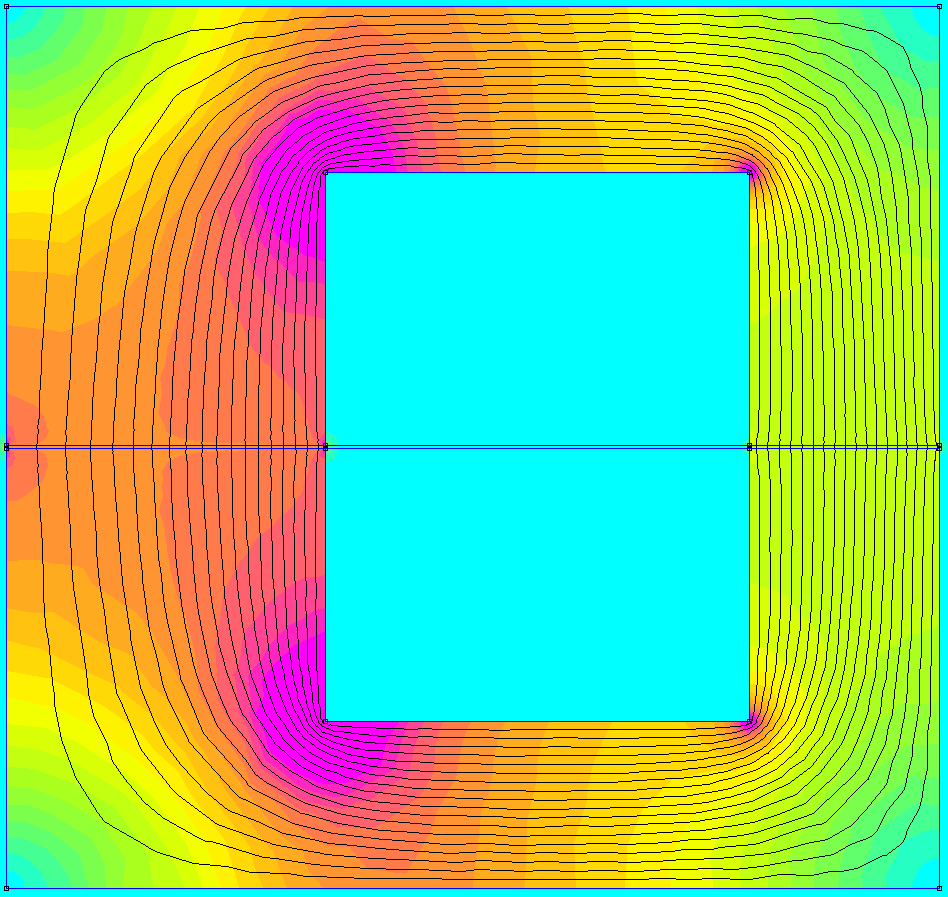
\includegraphics[width=0.45\linewidth]{saettigung_1}}\qquad
	\subfloat[Farbskala in Tesla]{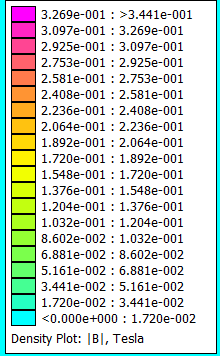
\includegraphics[width=0.25\linewidth]{saettigung_2}}
	\caption{Speichertransformator mit 0.1mm Abstand}
	\label{fig:saettigung}
\end{figure}
\newpage

Mit Hilfe der zweiten Simulation im FEMM soll der Koppelungsfaktor anhand der Formel \ref{eq:kopplungsfaktor} ermittelt werden. Um ihn berechnen zu können, benötigt man die Induktivität und die Gegeninduktivität.

\begin{figure}[H]
	\centering
	\subfloat[Strom durch primär Wicklung.]{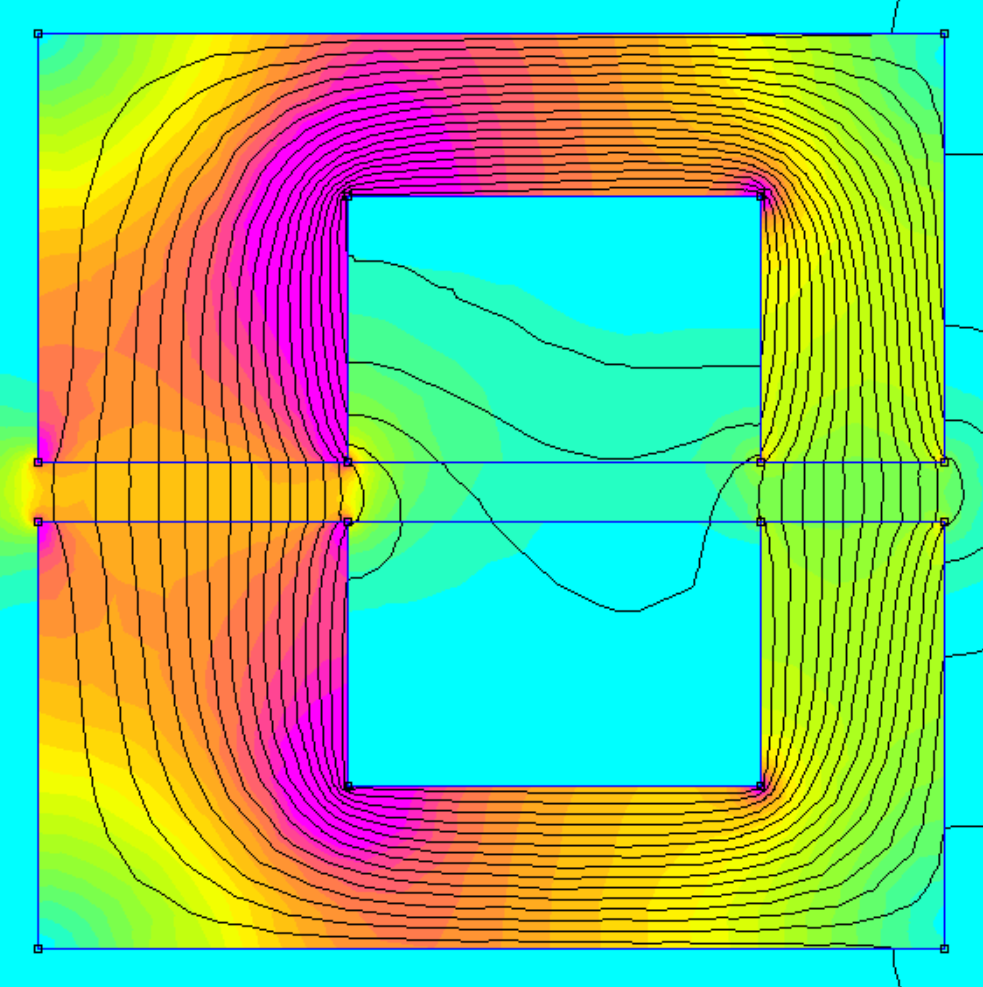
\includegraphics[width=0.45\linewidth]{femm_1.png}}\qquad
	\subfloat[Strom durch primär und sekundär Wicklung.]{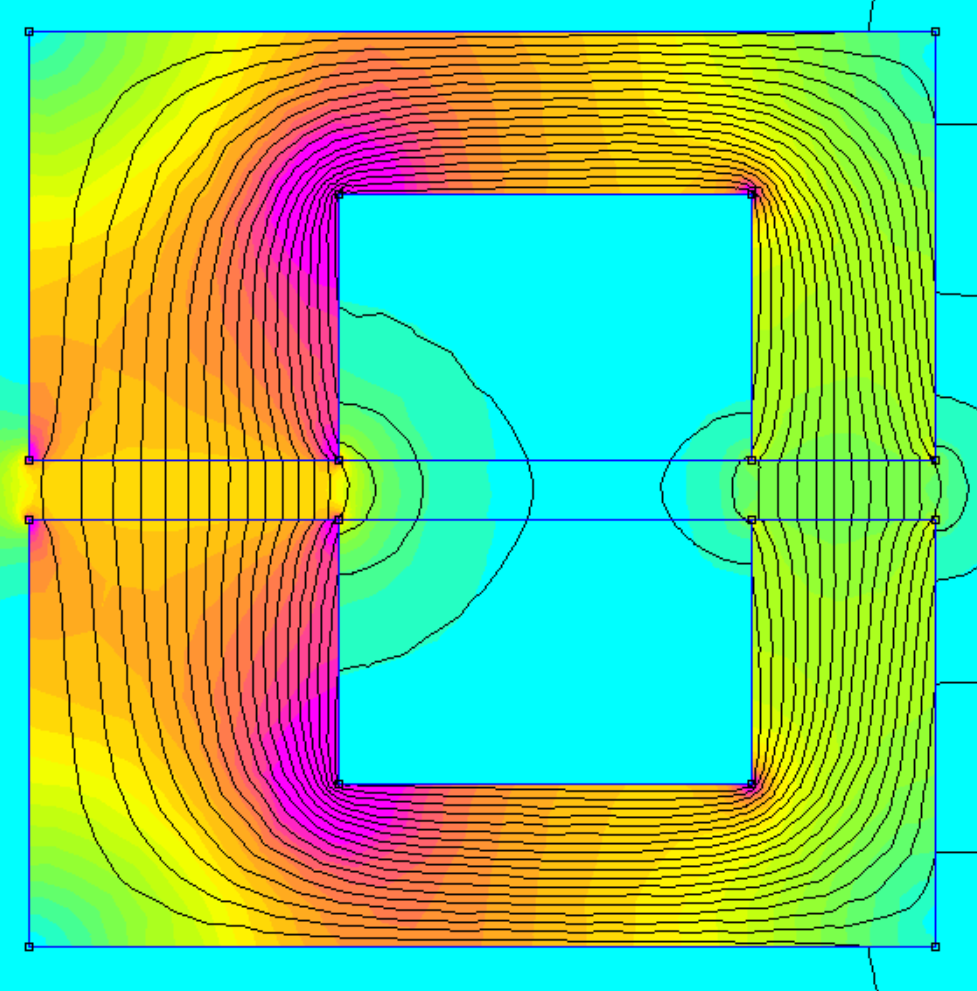
\includegraphics[width=0.45\linewidth]{femm_2.png}}
	\caption{Simulation des FEMM Models.}
	\label{fig:femmkopplung}
\end{figure}

In FEMM kann die Selbstinduktion der Primärspule simuliert werden, indem man einen Strom, wie in der Abbildung \ref{fig:femmkopplung} durch die Primärwicklung lässt. Mit dem ermittelten Fluss $ \Psi_{11}  $ und dem Strom $ I_{1} $ kann die Induktivität $ L_{1} $ wie folgt berechnet werden. Das Simulationstool übernimmt diese Rechnung und kann die Induktivität direkt ausgeben.\cite{femm}

\begin{equation}
L_{1}=\frac{\Psi_{11}}{I_{1}}
\label{eq:femm_l1}
\end{equation}

Mit der Formel \ref{eq:femm_M} wird die gesuchte Gegeninduktivität $ M $ berechnet.
Der dazu benötigte Fluss $ \Psi_{1} $ lässt sich in FEMM ermitteln indem man durch die Primär und Sekundärspule einen Strom fliessen lässt, wie in der Abbildung \ref{fig:femmkopplung}. \cite{femm}

\begin{equation}
M=\frac{\Psi_{1}-\Psi_{11}}{I_{1}}=\frac{\Psi_{12}}{I_{1}}
\label{eq:femm_M}
\end{equation}

Da $ L_{1} $ und $ L_{2} $ denselben Wert besitzen, kann man die Formel \ref{eq:kopplungsfaktor} vereinfachen, wodurch sich nun der Kopplungsfaktor $ k $ wie folgt definiert.

\begin{equation}
k=\frac{M}{\sqrt{L_{1}^{2}}}
\label{eq:kopplungsfaktor_neu}
\end{equation}

In der Tabelle \ref{tab:kopplung} sind die Resultate der Simulation eingetragen. In der letzten Spalte ist der Kopplungsfaktor mit der Formel \ref{eq:kopplungsfaktor_neu} berechnet. Die für die Berechnung benötigte Induktivität ist aus der Tabelle \ref{tab:windungen} aus der Spalte der simulierten Resultate entnommen worden. 

\begin{table}[h]
	\centering
	\begin{tabular}{>{\tt}C{2.0cm}| C{3cm} |  C{3cm} |  C{3cm} |  C{1.5cm}} 
		\normalfont\textbf{Frequenz} & \normalfont\textbf{Abstand} & \normalfont\textbf{$ \mathbf{\mathrm{\Psi_{11}}} $} & \normalfont\textbf{$ \mathbf{\mathrm{\Psi_{1}}} $} & \normalfont\textbf{k}\\ \hline\hline 
		\multirow{2}{*}{10 kHz} & \SI{0.1e-03}{m} & \SI{446.9e-06}{W} & \SI{889.2e-06}{W} &  \textbf{0.989}    \\ 
		& \SI{1e-03}{m} & \SI{583.3e-06}{W} & \SI{1100e-06}{W} & \textbf{0.934}     \\ \hline
		\multirow{2}{*}{20 kHz} & \SI{0.1e-03}{m} & \SI{ 251.5e-06}{W} & \SI{ 500.2e-06}{W} & \textbf{0.989}    \\ 
		       & \SI{1e-03}{m} & \SI{260e-06}{W}& \SI{502.1e-06}{W} &  \textbf{0.932}   \\ \hline
			\multirow{2}{*}{30 kHz} & \SI{0.1e-03}{m} & \SI{251.6e-06}{W} & \SI{500.4e-06}{W} & \textbf{0.988}     \\ 
		& \SI{1e-03}{m} & \SI{199.1e-06}{W} & \SI{384.5e-06}{W} &  \textbf{0.93}   \\ \hline
			\multirow{2}{*}{40 kHz} & \SI{0.1e-03}{m} & \SI{112.1e-06}{W} & \SI{222.7e-06}{W} &  \textbf{0.986}    \\ 
		& \SI{1e-03}{m} & \SI{146.5e-06}{W} & \SI{282.7e-06}{W} & \textbf{0.929}     \\ \hline
			\multirow{2}{*}{50 kHz} & \SI{0.1e-03}{m} & \SI{112.1e-06}{W} & \SI{222.7e-06}{W} &  \textbf{0.986}    \\ 
		& \SI{1e-03}{m} &\SI{102.02e-06}{W} & \SI{196.56e-06}{W}&  \textbf{0.926}   \\ \hline
	\end{tabular}
	\caption{Induktivität in Abhängigkeit der Schaltfrequenz }
	\label{tab:kopplung}
\end{table}

Der Kopplungsfaktor k beträgt etwas mehr als 0.9. Er wird grösser indem die Induktivität erhöht wird. Der beste Kopplungsdoktor ist daher bei einer Frequenz von 10kHz und einem Abstand von 0.1mm. 


\paragraph{Schaltung}
Das Ziel der Simulation ist es, verschiedene Erkenntnisse über die Schaltung zu erhalten, wie der Wirkungsgrad, der Ausgangsstrom oder die Ausgangsspannung. Die Schaltung ist im LTspice aufgebaut. Die Bauteile, welche für den Flyback-Converter benötigt werden, wurden anhand der Dimensionierung ausgesucht.

Der Speichertransformator wurde für 20kHz ausgelegt. Dies bringt mehrere Vorteile mit sich. Als erstes hört man diese Frequenz nicht mehr, was das Arbeiten mit dem Testaufbau einiges angenehmer macht. Beim Abstand von 0.1mm hat die berechnete Induktivität fast die kleinste Differenz zur simulierten Induktivität einer ganzen Windung. Zum Zweiten hat die Spule nicht nur zwei Windungen und bietet etwas mehr Flexibilität.

Der Widerstand kann mit der Formel \ref{eq:Leistung} berechnet werden indem sie nach R umgeformt wird. 

\begin{equation}\label{eq:Widerstand}
R= \frac{U_{2}\!^{2}}{P}=\frac{48^{2}V}{300 W} = 7.68\Omega
\end{equation}

In der Abbildung \ref{fig:LT_schema} ist der Flyback-Converter mit einer Zener-Snubber-Schaltung aufgebaut. Mit dieser Schaltung sind die nachfolgenden Simulationen durchgeführt worden.

\begin{figure}[H]
	\centering
	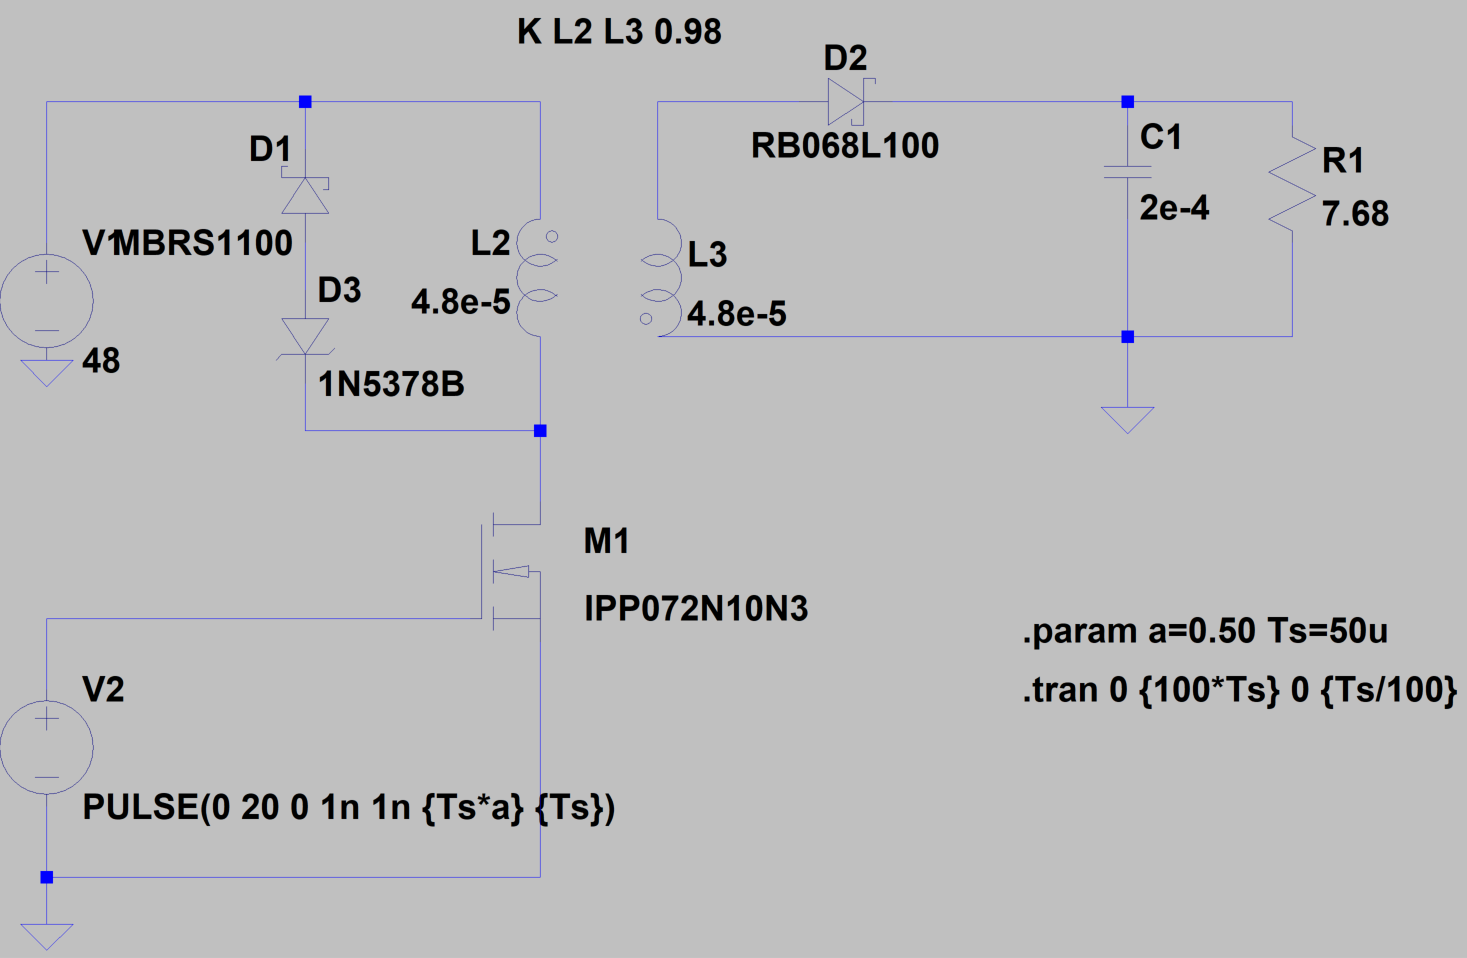
\includegraphics[width=1\linewidth]{LT_schaltung}
	\caption{Flyback-Converter im LTspice}\label{fig:LT_schema}
\end{figure}

Der Strom und die Spannung am Widerstand R1 sind in der Abbildung \ref{fig:ausgangsstrom} simuliert. Der Mittelwert und der RMS-Wert sind in der Tabelle \ref{tab:ausgang} eingetragen.

\begin{table}[h]
	\centering
	\begin{tabular}{>{\tt}C{2.3cm}|  C{3cm}|  C{3cm}} 
		\normalfont\textbf{Grösse} & \normalfont\textbf{Mittelwert} & \normalfont\textbf{RMS-Wert} \\ \hline\hline 
		Spannung & 47.6V & 48.4V   \\ \hline
		Strom & 6.2A &   6.3A   \\ \hline
		Leistung & 304.98W &      \\ \hline
	\end{tabular}
	\caption{Resultate der Simulation}
	\label{tab:ausgang}
\end{table}

Die Schaltung hat einen Wirkungsgrad von 52\%, der sich wie folgt berechne lässt. 

\begin{equation}\label{eq:wirkungsgrand}
\eta=\frac{P_{ab}}{P_{zu}}=\frac{304.79W}{585.52W} = 0.52
\end{equation}

\begin{figure}[H]
	\centering
	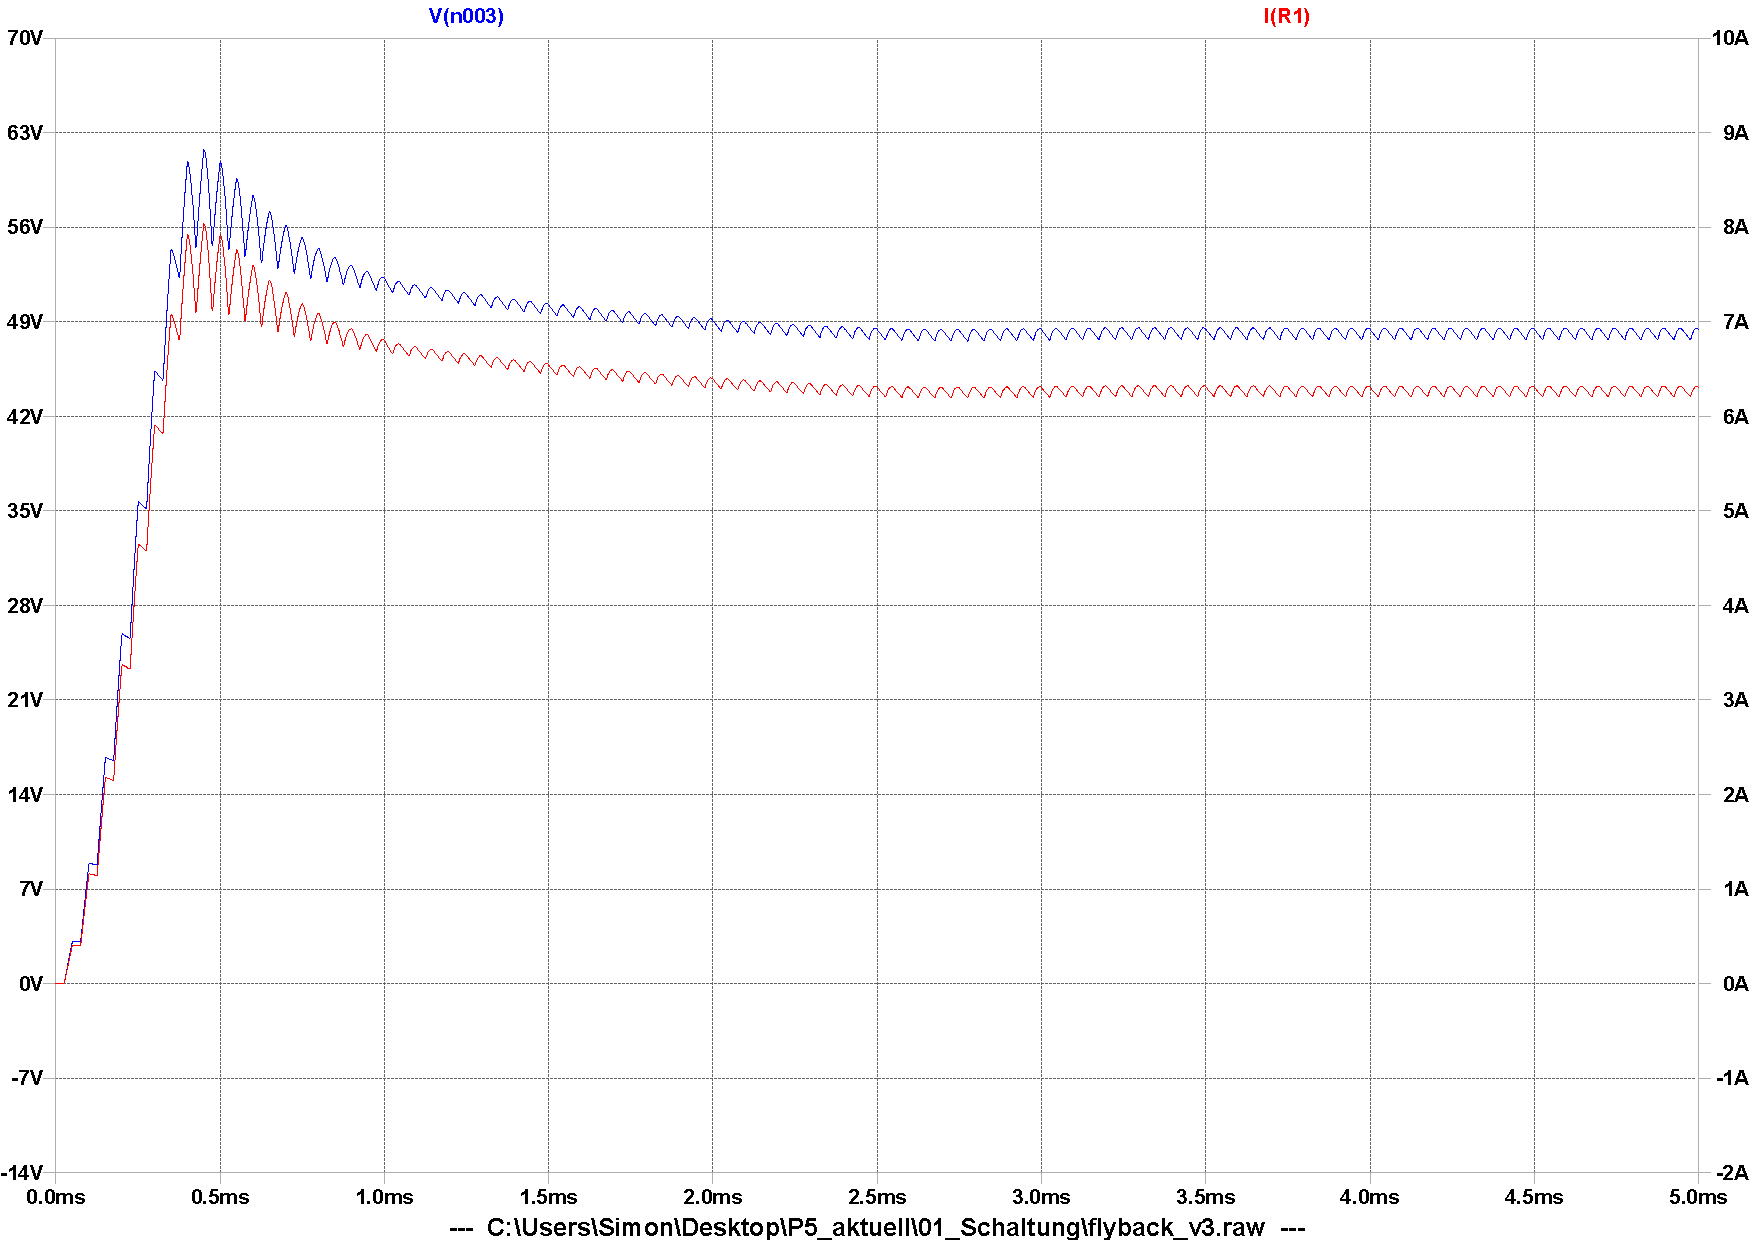
\includegraphics[width=0.7\linewidth]{flyback_v3_spannung}
	\caption{Strom (rot) und Spannung (blau) über dem Widerstand R1 }\label{fig:ausgangsstrom}
\end{figure}

Der Strom in der Spule L1 und der in Strom der Spule L2 mit dem PWM-Signal sind in der Abbildung \ref{fig:spule} Plot a) dargestellt. Dieser Plot kann mit der Abbildung \ref{fig:kurven} verglichen werden. Auch in der Simulation werden die beiden Strom-Dreiecke ersichtlich. Zusätzlich zu den Strömen ist die Spannung über der Spule L1  im Plot b abgebildet.

\begin{figure}[H]
	\centering
	\subfloat[Strom durch die Primär-Spule (blau) und Strom durch die Sekundär-Spule (rot) mit dem PWM-Signal (grün)]{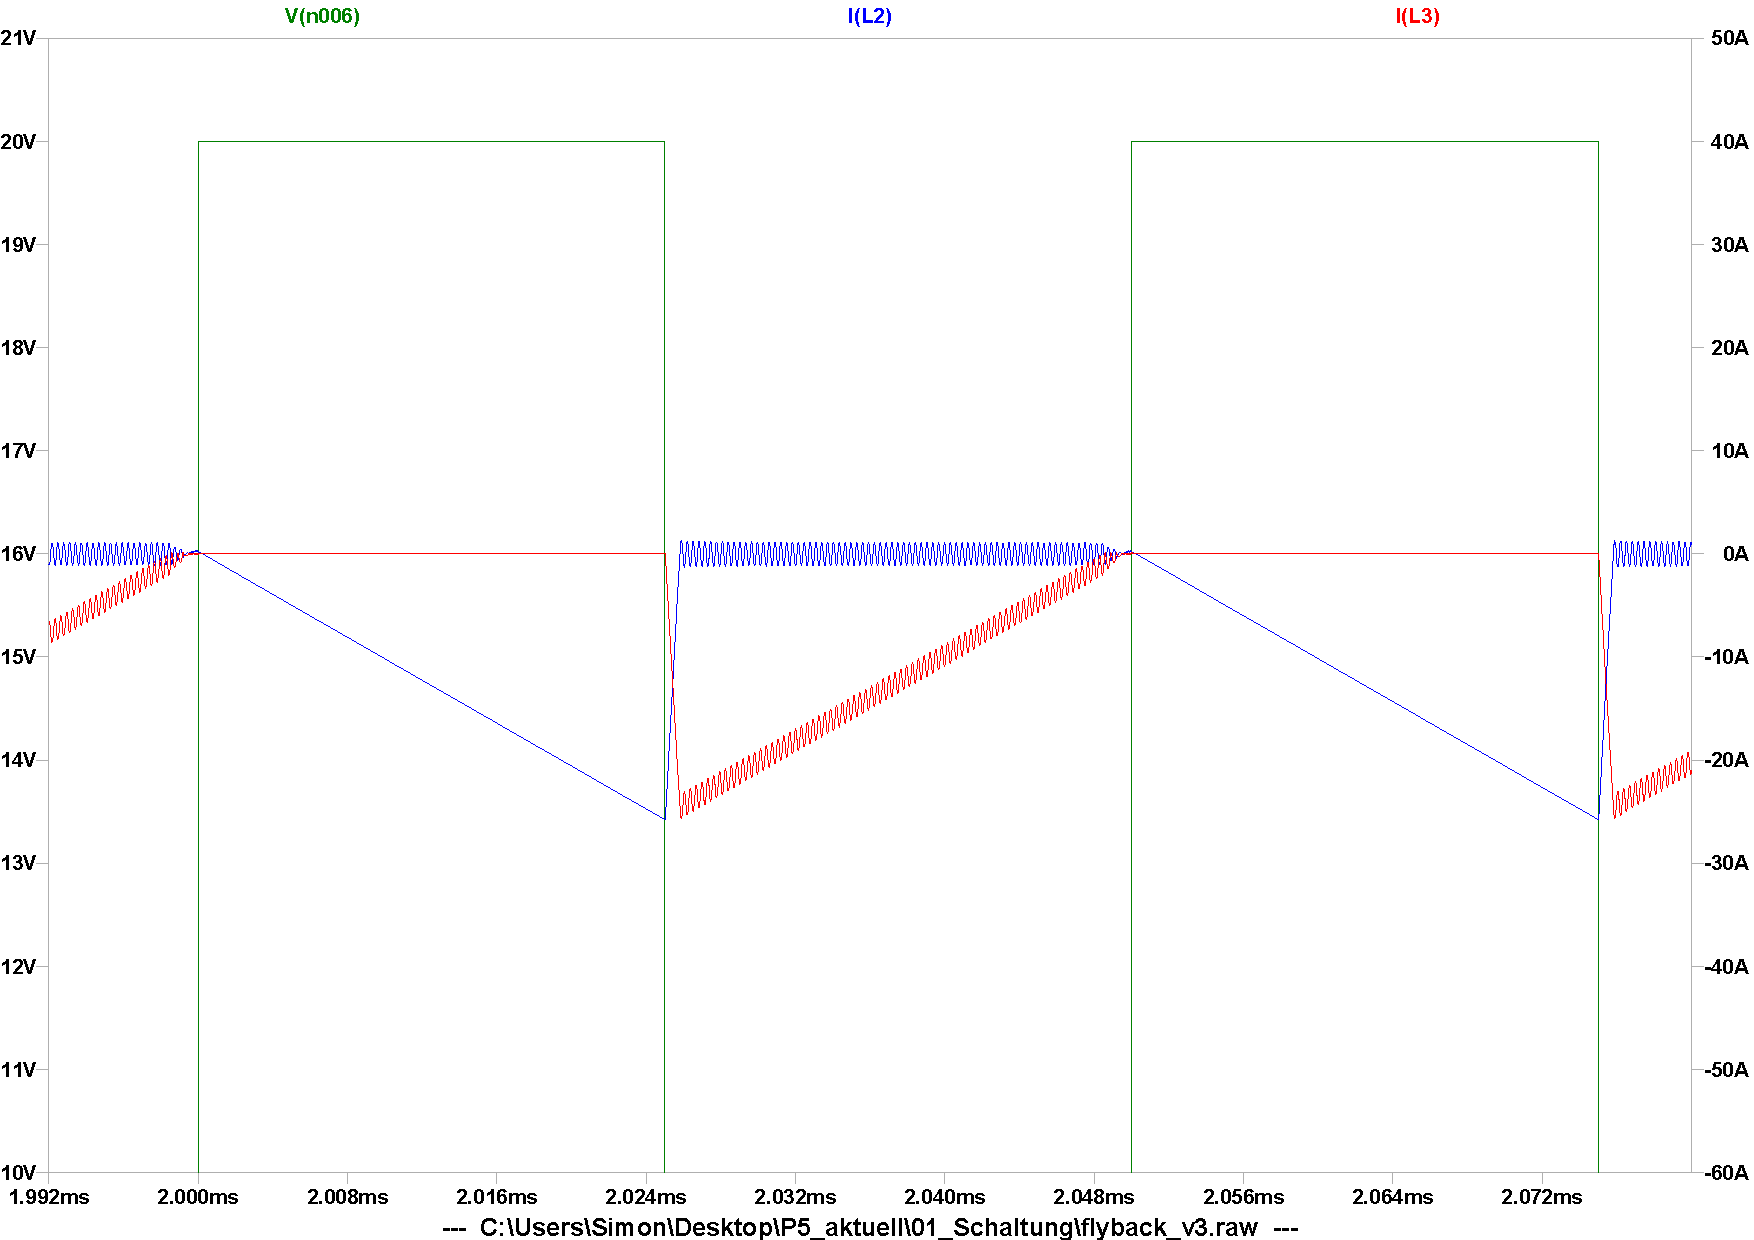
\includegraphics[width=0.47\linewidth]{flyback_v3_spule1}}\qquad
	\subfloat[Strom durch die Primär-Spule (blau) und Strom durch die Sekundär-Spule (rot) mit der Spannung über der Primär-Spule (grün)]{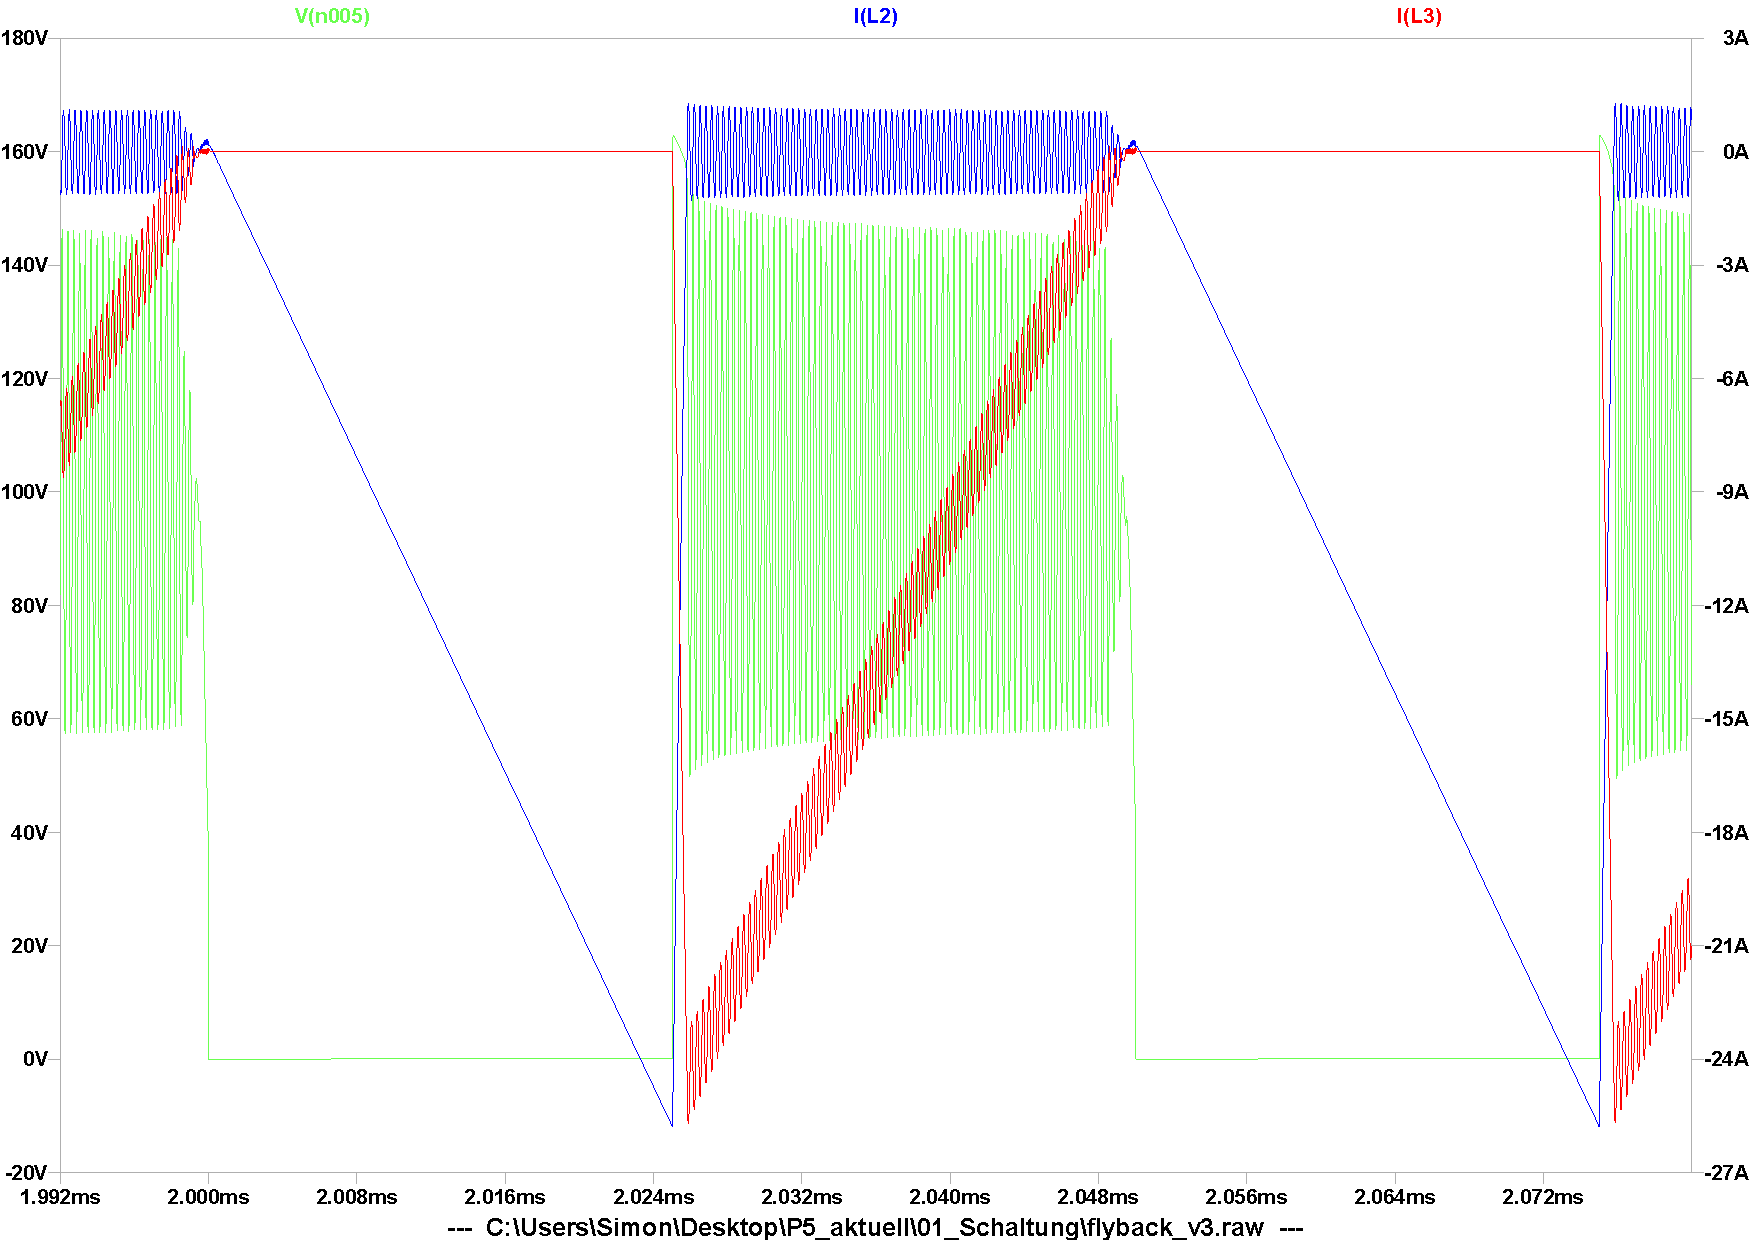
\includegraphics[width=0.47\linewidth]{flyback_v3_spule2}}
	\caption{Speichertransformator mit 0.1mm Abstand}
	\label{fig:spule}
\end{figure}

In der Abbildung wird der Strom und die Spannung über der Spule mit und ohne Snubber verglichen.

\begin{figure}[H]
	\centering
	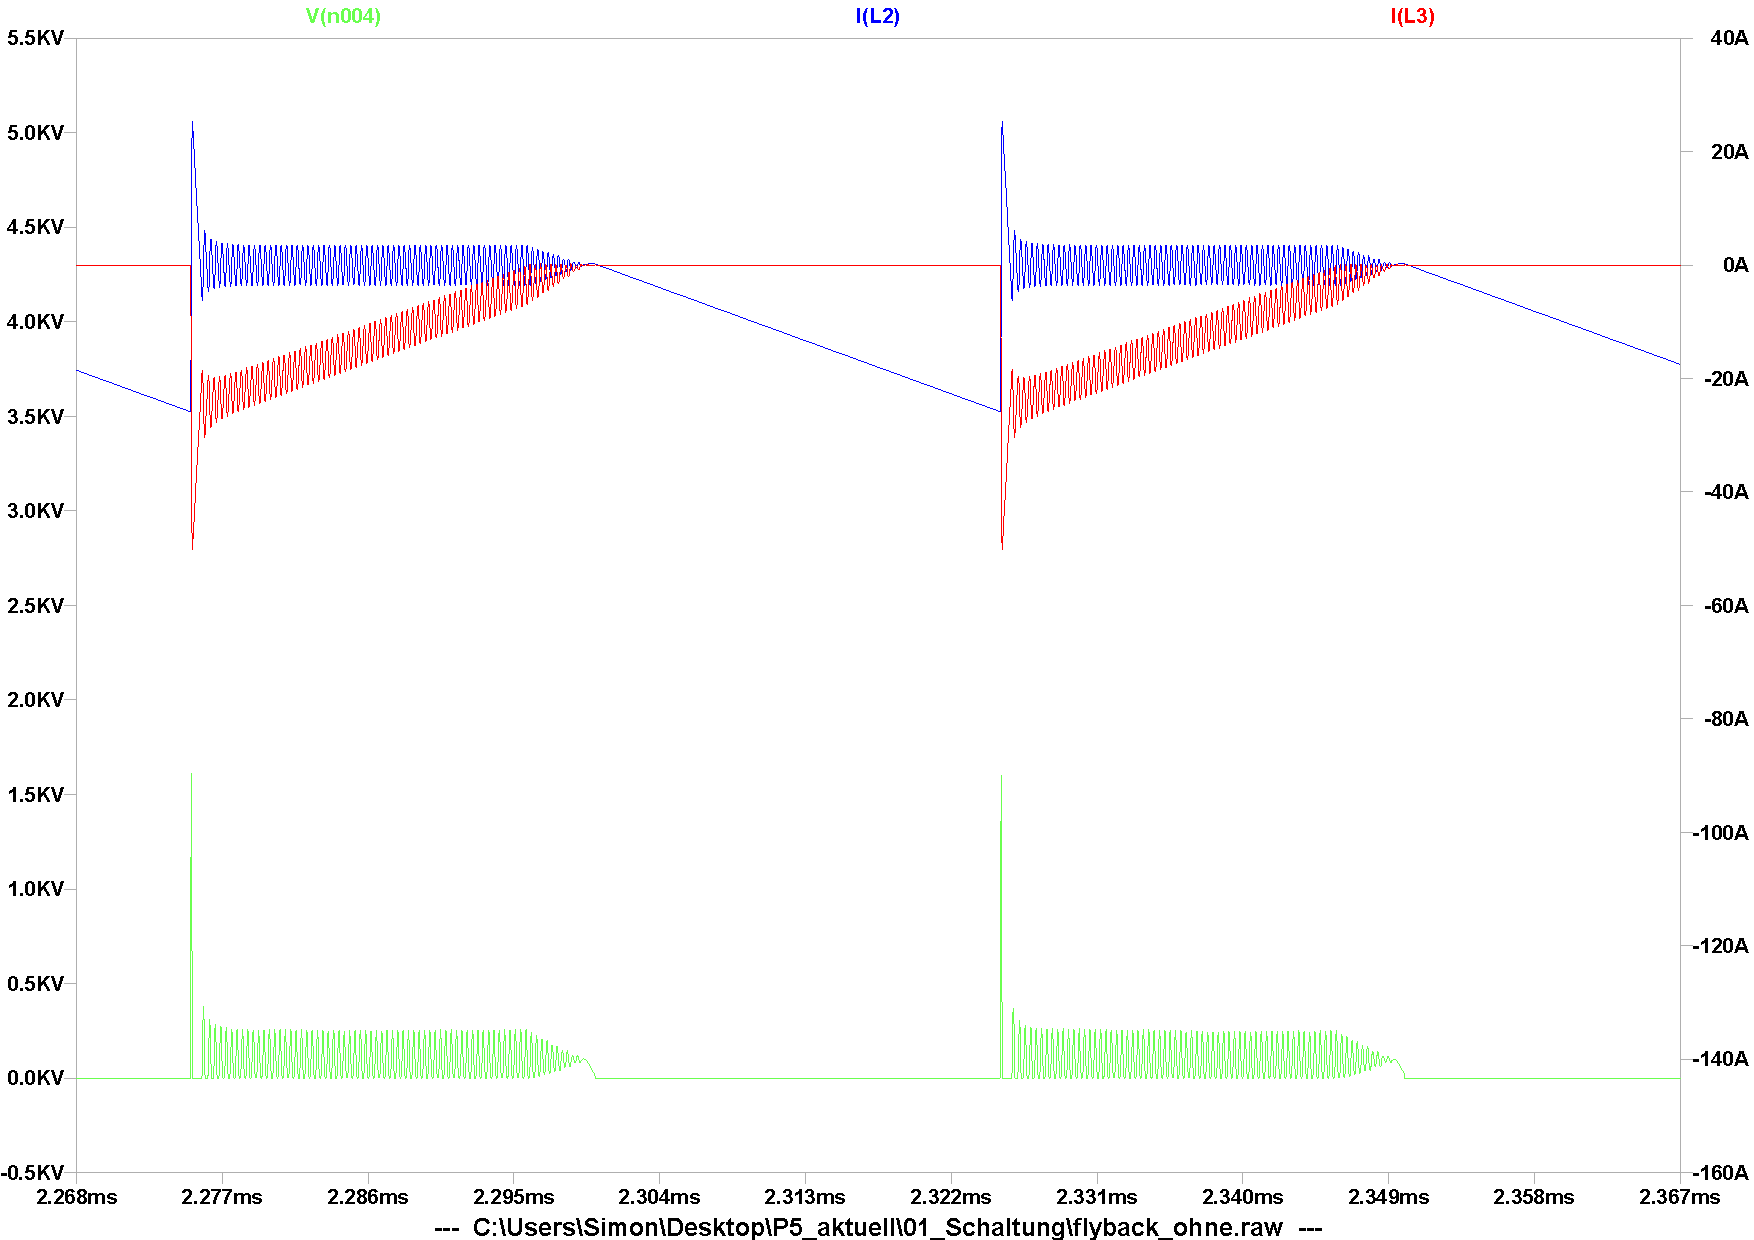
\includegraphics[width=0.7\linewidth]{flyback_ohne}
	\caption{Strom durch die Primär-Spule(blau) und Storm durch die Sekundär-Spule (rot) mit der Spannung über der Primär-Spule (grün) }\label{fig:LT_snubber}
\end{figure}

In der Abbildung \ref{fig:LT_snubber} steigt die Spannung über der Primär-Spule ohne das Snubber-Glied auf eine Spannung von 1.5kHz. Die beiden Strom-Dreiecke haben ein erhöhtes Schwingen und einen hohen Pick. 

Mit der Simulation in LTspice kann auch die Verlustleistung der Halbleiter ermittelt werden. Die Resultate sind in der Tabelle \ref{tab:LT_verlsutleistung} aufgeführt.

\begin{table}[h]
	\centering
	\begin{tabular}{>{\tt}C{2.3cm}| C{6cm}} 
		\normalfont\textbf{Bauteil} & \normalfont\textbf{Mittlere Verlustleistung} \\ \hline\hline 
		MOSFET M1 & 3.84W  \\ \hline
		Diode D1 & 197mW  \\ \hline
		Diode D2 & 26.47W \\ \hline
		Z-Diode D3 & 23.16W  \\ \hline
	\end{tabular}
	\caption{Resultate der Simulation}
	\label{tab:LT_verlsutleistung}
\end{table}

\subsection{Testaufbau}
Der Testaufbau ist in das Konstruieren des Speichertransformators und in das Erstellen der Schaltung unterteilt. 

Der Speichertransformator besteht aus zwei Ferrit-Schalenkerne, zwei Spulenkörper und  lackisoliertem 1.5mm Kupferdraht. Der Spulenkörper wird benötigt um die Wicklungen wie in Abbildung \ref{fig:aufbau_spule} herzustellen. Beide Wicklungen wurden mit 4 Windungen hergestellt.
Zwischen den beiden Schalenkernen wurde mit einem Klebband ein Abstand von 0.1mm realisiert. Die beiden Schalenkerne wurden zu einem Speichertransformator zusammengeklebt.

\begin{figure}[H]
	\centering
	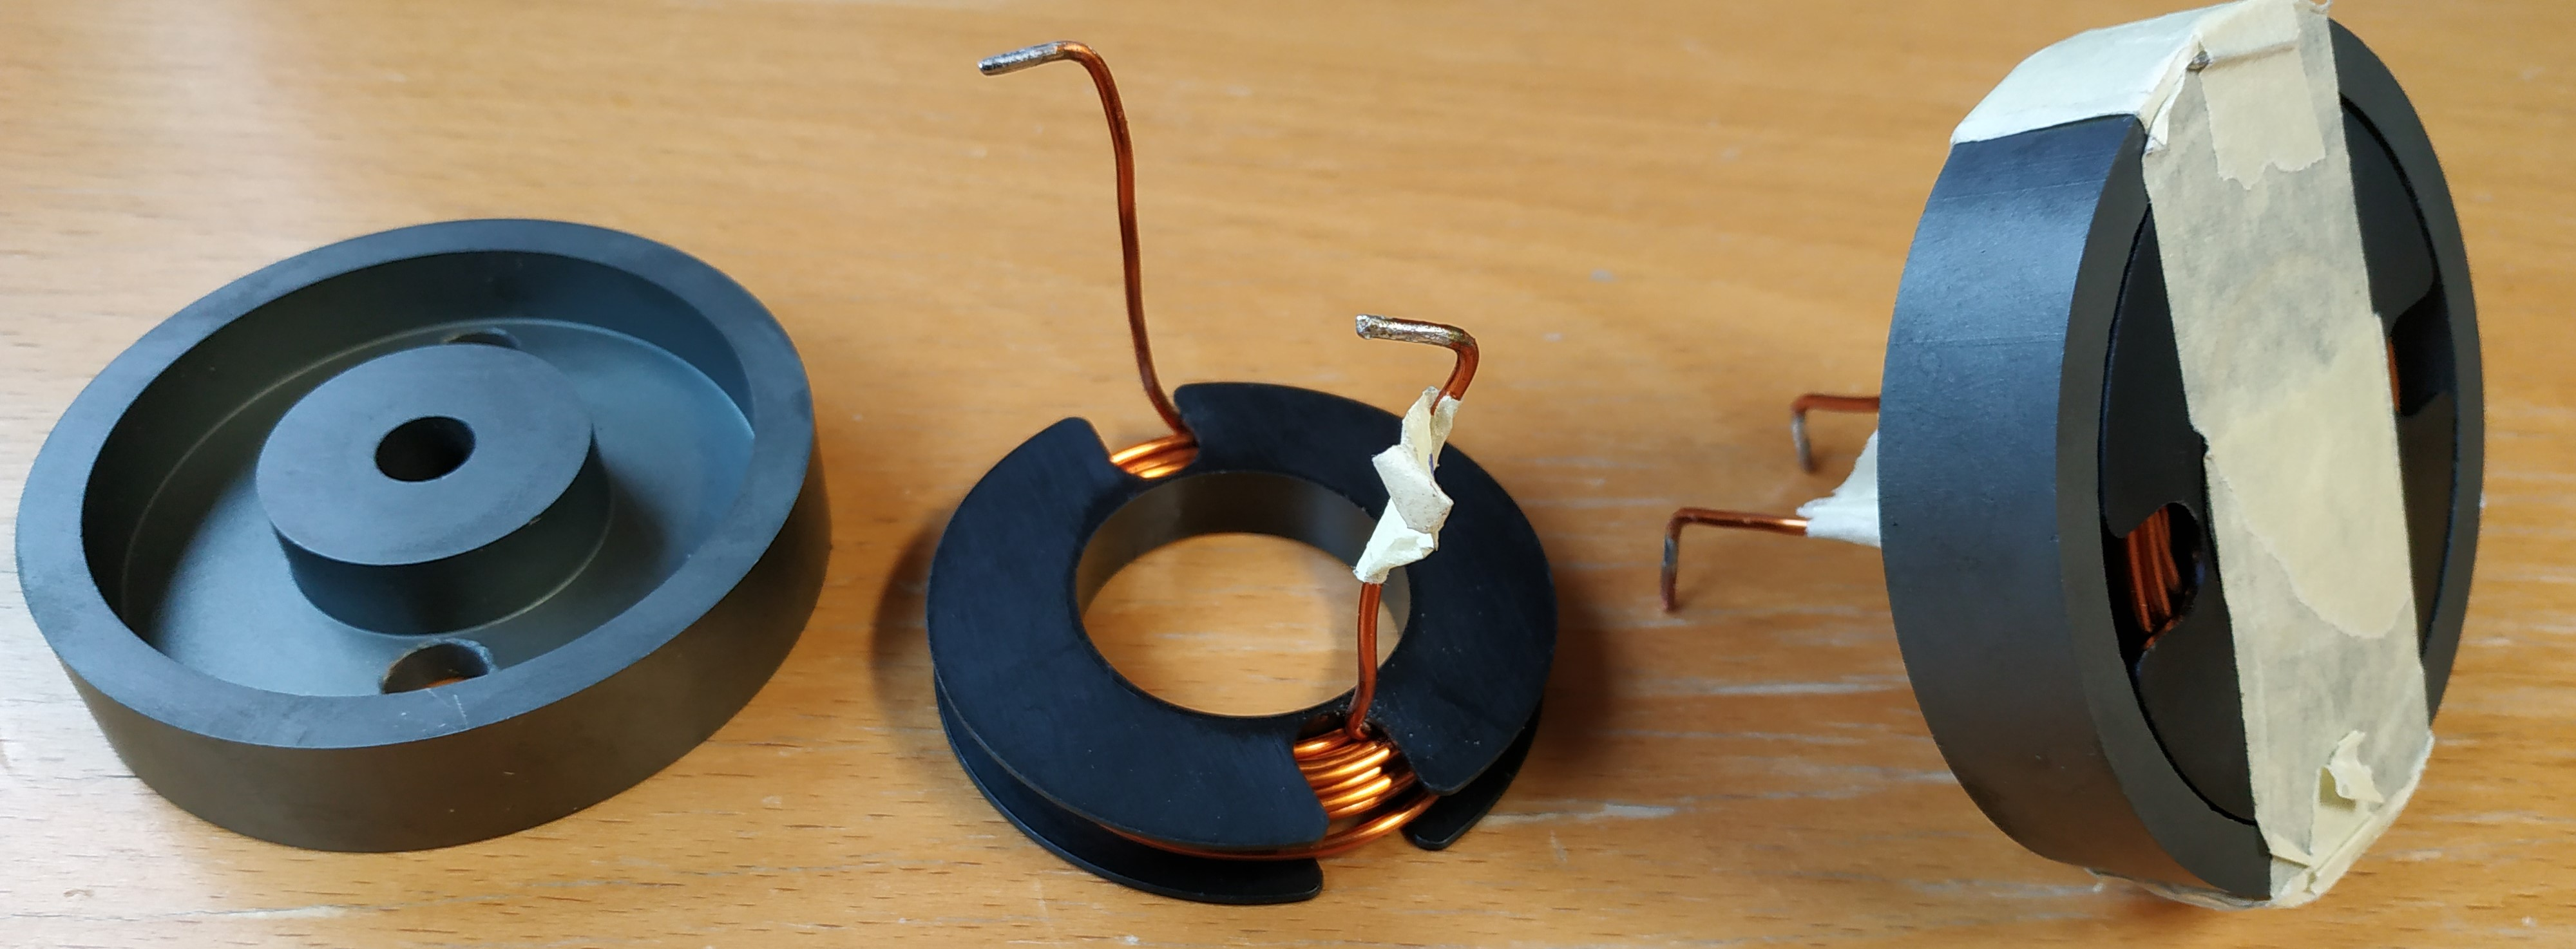
\includegraphics[width=0.7\linewidth]{spule}
	\caption{Testaufbau des Flyback-Converters}\label{fig:aufbau_spule}
\end{figure}

Der Flyback-Converter besteht aus einer Primär- und einer Sekundär-Schaltung. Beide Schaltungen sind anhand der Simulation gelayoutet und aufgebaut worden. In der Abbildung \ref{fig:testaufbau} ist der Testaufbau dargestellt. Von links nach rechts besteht er aus der Primär-Schaltung, dem Speichertransformator (zwei Schalenkerne), der Senkundär-Schaltung und dem Widerstand.

\begin{figure}[H]
	\centering
	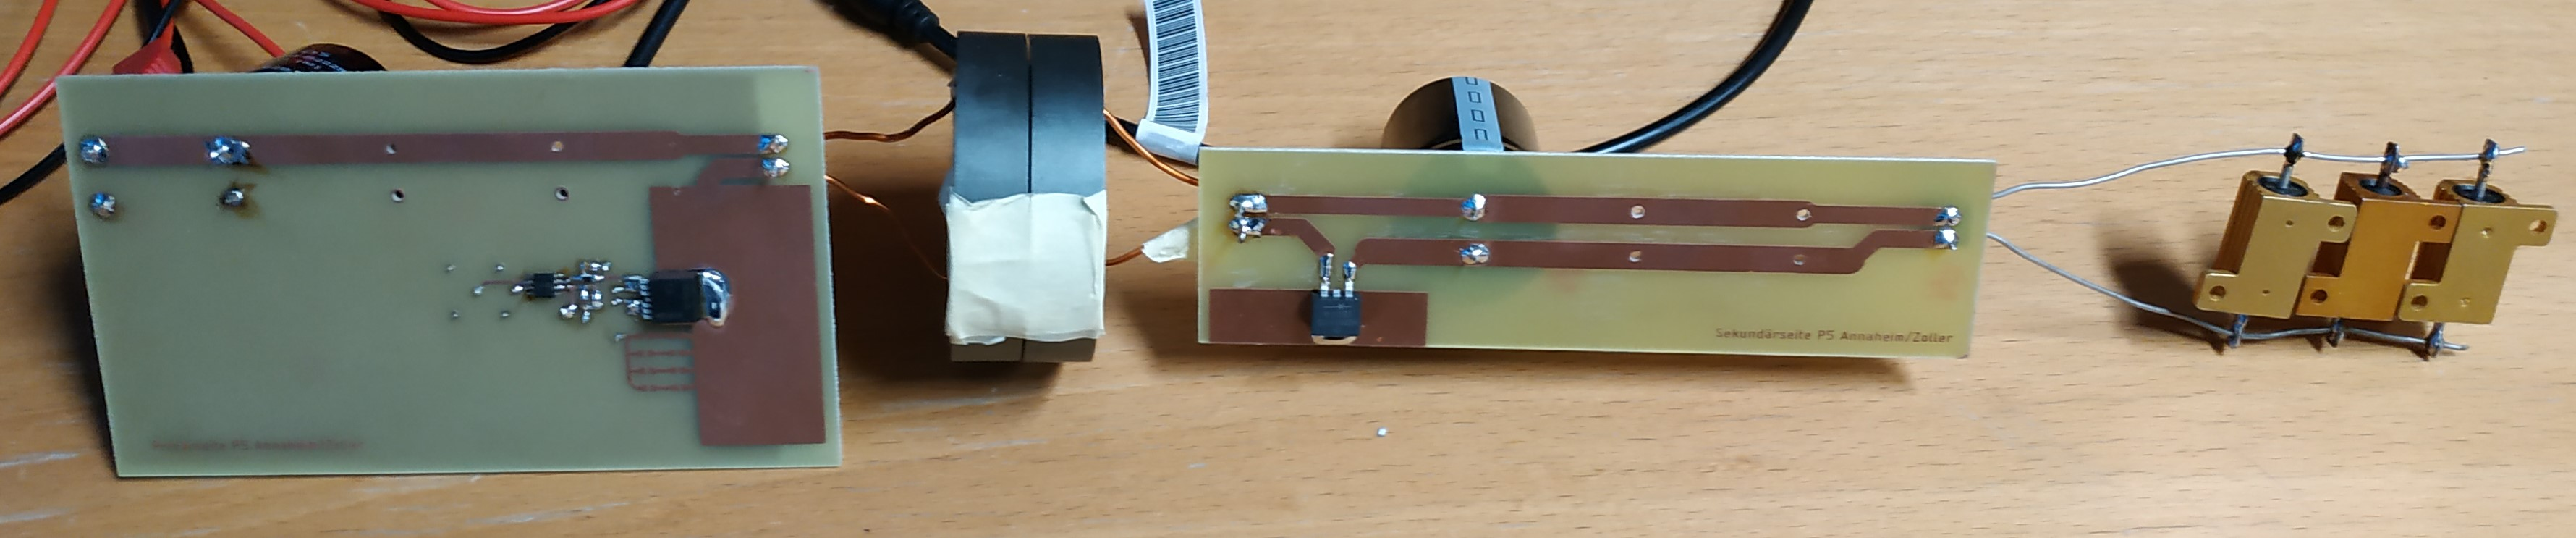
\includegraphics[width=0.9\linewidth]{flyback_aufbau}
	\caption{Testaufbau des Flyback-Converters}\label{fig:testaufbau}
\end{figure}

\subsection{Validierung}
In der Validierung wird der Testaufbau mit der Simulation verglichen. Damit soll die Simulationen der Induktivität und des Kopplungsfaktor mit FEMM  überprüft werden. Der gesamte Testaufbau mit der Schaltung und dem Speichertransformator wird mit der Simulation in LTspice verglichen.

\paragraph{Messung der Induktivität}
Mit dieser Messung soll überprüft werden, ob die simulierte Induktivität mit der Realität übereinstimmt. In der ersten Messung wurde ein Transformator mit 14 Windungen aufgebaut und mit einer Frequenz von 20kHz betrieben. In der Abbildung \ref{fig:mess_ind} sind die Resultate dargestellt. Die Simulation ergab eine Induktivität von $ \SI{7.8e-05}{H} $ und die Messung von $ \SI{7.9e-05}{H} $. Dies ergibt eine Abweichung von etwa 2\%. 

Bei einer zweiten Messung besteht der Transformator aus 4 Windungen, einem Abstand von 0.1mm und derselben Frequenz wie in der ersten Simulation. Die gemessene Induktivität beträgt $ \SI{3.7e-05}{H} $ bis zu $ \SI{5.1e-05}{H} $, je nach dem wie stark die beiden Schalenkerne zusammengedrückt sind. In der Simulation wurde eine Induktivität $ \SI{7.45e-05}{H} $ von ermittelt. Die Abweichung beträgt etwa 50\% bis 70\%. 

\begin{figure}[H]
	\centering
	\subfloat[Simulation in FEMM]{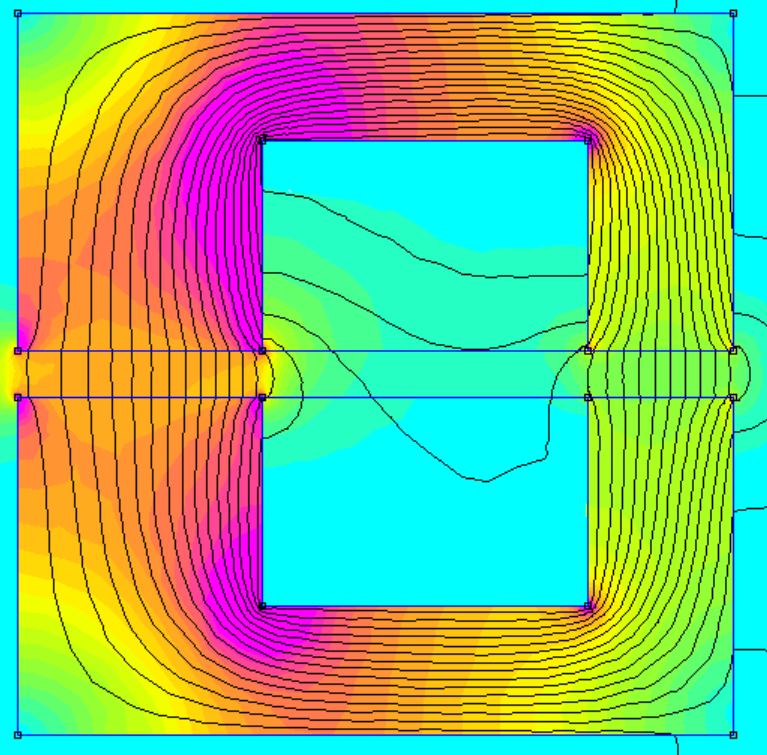
\includegraphics[width=0.4\linewidth]{vali_indukivitaet}}\qquad
	\subfloat[Messung der Induktivität ]{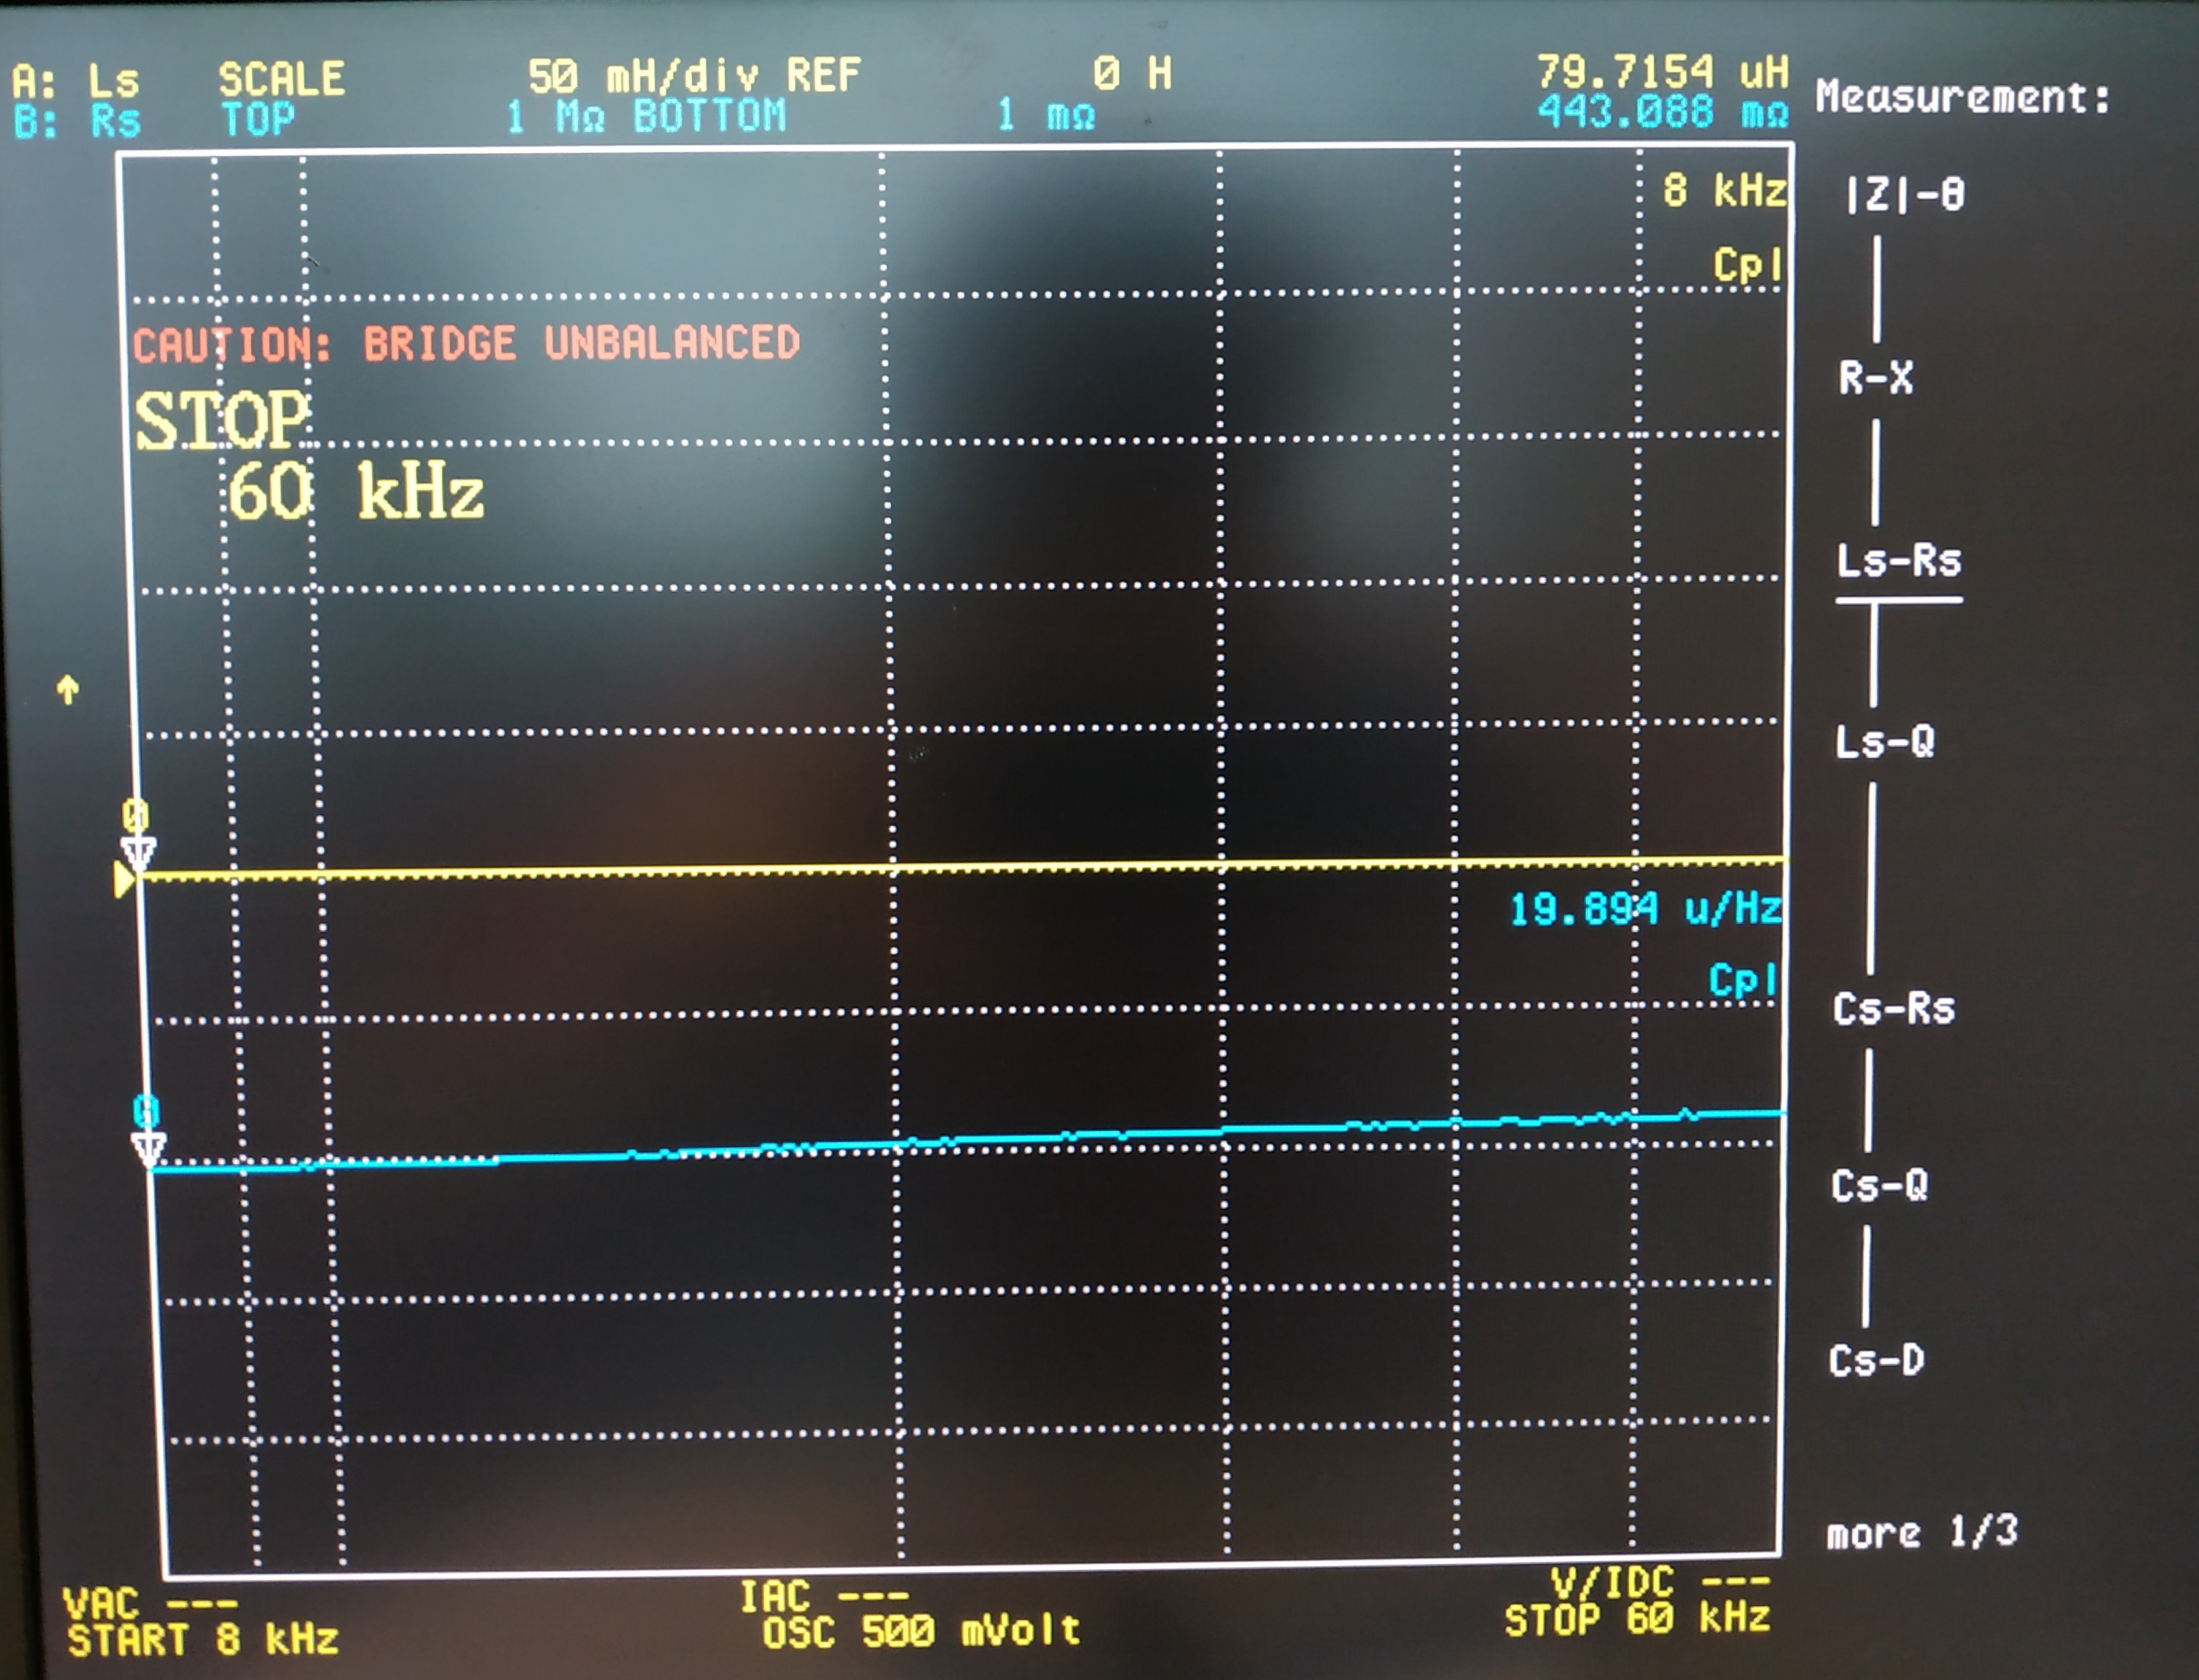
\includegraphics[width=0.47\linewidth]{induktivitaet}}
	\caption{Resultate der Induktivität}
	\label{fig:mess_ind}
\end{figure}

\paragraph{Messung des Kopplungsfaktor}
Der Kopplungsfaktor kann gemessen werden, indem die Induktivität im Leerlauf und bei kurzgeschlossener sekundärer Windung gemessen wird. In die Formel \ref{eq:mes_k} können die beiden ermittelten Induktivitäten eingesetzt werden um den Kopplungsfaktor zu berechnen.

\begin{equation}\label{eq:mes_k}
k = \sqrt{1-\frac{L_{kurz}}{L_{offen}}}
\end{equation}

Für den Transformator mit 4 Windungen berechnet sich der Kopplungsfaktor wie folgt:

\begin{equation}\label{eq:berechnung_k1}
k = \sqrt{1-\frac{\SI{3.2e-06}{H}}{\SI{37e-06}{H}}}=0.95
\end{equation}

\begin{equation}\label{eq:berechnung_k2}
k = \sqrt{1-\frac{\SI{3.2e-06}{H}}{\SI{51e-06}{H}}}=0.97
\end{equation}

Der Transformator hat einen Kopplungsfaktor von 0.95 bis 0.97 je nach Induktivität. Dieser weicht stark von dem simulierten Kopplungsfaktor von 0.989 ab. Da die Kopplung zwischen den Spulen kleiner ist, als simuliert, ist die Streuinduktivität höher als erwartet. Dies hat Auswirkungen auf die Schaltung. Es wird weniger Energie übertragen und die nicht übertragene Leistung muss auf der Primärseite abgebaut werden.  

\paragraph{Messungen am Testaufbau}
Da der Kopplungsfaktor des Speichertransformator sehr schlecht ist, konnte der Testaufbau nicht mit der vollen Leistung getestet werden. Die folgenden Messungen wurden mit einer Eingangsspannung von 15 Volt und einem Strom von 2 Ampere durchgeführt.   

In der Abbildung \ref{fig:mess_ströme} sind die Messresultate der Ströme über den Spulen dargestellt. Die Messungen kann mit der Abbildung \ref{fig:kurven} und der Abbildung \ref{fig:spule} verglichen werden. Ein Vergleich zeigt, dass der Strom in der Sekundärspule (gelb) gedämpfter zum Primär-Strom (violett) ist und in der Hälfet der Ausschaltdauer des MOSFETs auf Null geht. In dem Plot b) ist zusätzlich zu den Strömen die Spannung (grün) über der Primärspule gemessen. Die Spannung schwingt stärker sobald der Sekundär-Strom auf Null ist. Zusätzlich steigt die Spannung kurz auf über 160V an. 

\begin{figure}[H]
	\centering
	\subfloat[Messung der Ströme über den Spulen und des PWM-Signals]{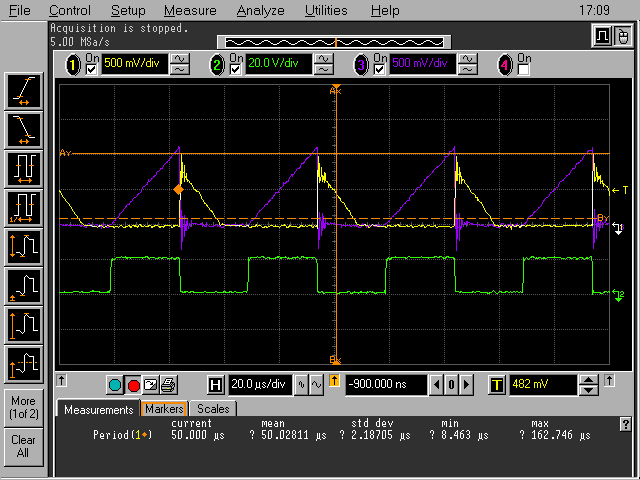
\includegraphics[width=0.47\linewidth]{Spulenstrom_mitpwm}}\qquad
	\subfloat[Messung der Induktivität ]{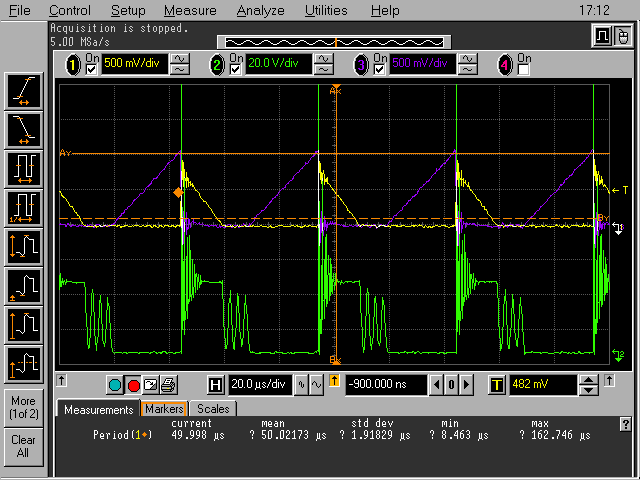
\includegraphics[width=0.47\linewidth]{Spulenstrom_mitspannung}}
	\caption{Resultate der Induktivität}
	\label{fig:mess_ströme}
\end{figure}


\todo[inline]{-Wirkungsgrad}